%Plate In A Newtonian Fluid
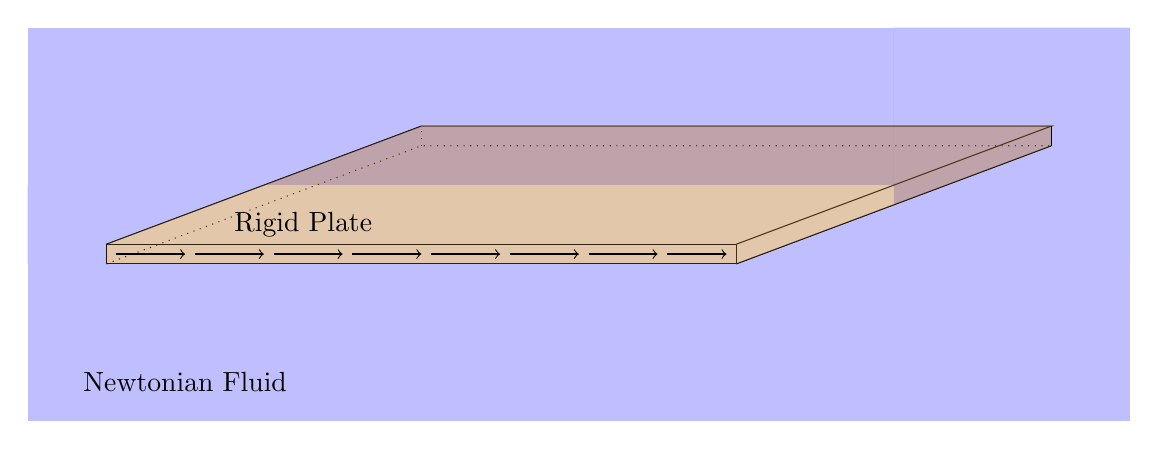
\begin{tikzpicture} 
	\path [fill, color=blue, opacity=0.25] (0,1) -- (14,1) -- (14,-1) -- (0, -1) -- cycle;
	\path [fill, color=blue, opacity=0.25] (9,1) -- (11, 1.75) -- (11, 4) -- (14, 4) -- (14,1) -- cycle;
	\path [fill, color=blue, opacity=0.25] (0,1) -- (1,1) -- (1,1.25) -- (3,2) -- (0,2) -- cycle;
	\path [fill, color=blue, opacity=0.25] (0,2) -- (0,4) -- (11,4) -- (11,2) -- cycle;
	\path [fill, color=brown, opacity=0.25] (1,1) -- (9,1) -- (9,1.25) -- (1, 1.25) -- cycle;	
	\draw (1,1) -- (9,1) -- (9,1.25) -- (1, 1.25) -- cycle;
	\draw [dotted] (1,1) -- (5,2.5) -- (13, 2.5);
	\draw (13,2.5) -- (9,1);
	\draw (1,1.25) -- (5,2.75) -- (13, 2.75) -- (9, 1.25);
	\path [fill, color=brown, opacity=0.25] (1,1.25) -- (5,2.75) -- (13, 2.75) -- (9, 1.25) -- cycle;
	\path [fill, color=brown, opacity=0.25] (1,1) -- (1,1.25) -- (5,2.75) -- (5,2.5) -- cycle;
	\path [fill, color=brown, opacity=0.25] (5,2.5) -- (5,2.75) -- (13,2.75) -- (13,2.5) -- cycle;
	\path [fill, color=brown, opacity=0.25] (9, 1) -- (9,1.25) -- (13,2.75) -- (13,2.5) -- cycle;
	\path [fill, color=brown, opacity=0.25] (1,1) -- (5,2.5) -- (13, 2.5) -- (9, 1) -- cycle;
	\draw (13,2.75) -- (13, 2.5);
	\draw [dotted] (5,2.5) -- (5,2.75);
 	\draw [->] (1.125,1.125) -- (2, 1.125);
 	\draw [->] (2.125, 1.125) -- (3, 1.125);
 	\draw [->] (3.125, 1.125) -- (4, 1.125);
 	\draw [->] (4.125, 1.125) -- (5, 1.125);
 	\draw (2,-0.5) node {Newtonian Fluid};
 	\draw (3.5,1.5) node {Rigid Plate};
 	\draw [->] (5.125, 1.125) -- (6, 1.125);
 	\draw [->] (6.125, 1.125) -- (7, 1.125);
 	\draw [->] (7.125, 1.125) -- (8, 1.125);
 	\draw [->] (8.125, 1.125) -- (8.875, 1.125);
% 	\path [fill, color=blue, opacity=0.5] (0,2) -- (14,2) -- (14,5) -- (0, 5) -- cycle;
\end{tikzpicture}
